\documentclass{article}
\usepackage{multicol}
\usepackage{graphicx}% Include figure files
\usepackage{dcolumn}% Align table columns on decimal point
\usepackage{bm}% bold math
\usepackage{hyperref}% add hypertext capabilities
\usepackage{booktabs}
\usepackage{listings}
\usepackage{mathtools}
\usepackage{amsmath}
\renewcommand{\abstractname}{\vspace{-\baselineskip}}
\bibliographystyle{plain}
\usepackage[utf8]{inputenc}
\usepackage{verbatim} %for å inkludere filer med tegn LaTeX ikke liker
\usepackage{mathpazo}
\usepackage{float}
\usepackage{algpseudocode}
\newcommand\numberthis{\addtocounter{equation}{1}\tag{\theequation}}
\usepackage[left=20mm,right=20mm,top=33.95mm,bottom=33.95mm]{geometry} 
% Justerer bredden på columns.
\setlength{\columnsep}{1cm}

\begin{document}

\title{Simulation of the two-dimensional Ising model}
\author{Sebastian Amundsen, Marcus Berget and Andreas Wetzel}

\maketitle

\begin{abstract}
We have simulated the Ising model in two dimensions using periodic boundary conditions. The simulation was done using the metropolis algorithm which is based on Monte Carlo sampling. First we tested the simulation using a $2 \times 2$ sized lattice. The computed expectation values for this system had a very small deviation from the analytical ones, indicating that the code worked. The burn-in time for this system was estimated to be $\tau=9\times10^4$ Monte Carlo cycles. We continued by extending the lattice size to $20 \times 20$. We estimated the burn-in time of this system to be $\tau = 1\times10^5$ Monte Carlo cycles. Finally, we studied the critical temperature of the phase transition of the Ising model. We computed the critical temperature to be $T_C=2.266$ J/k, which is very close to the analytical value of 2.269 J/k
\end{abstract}

\begin{multicols}{2}

\section{Introduction}
There are many different models for simulating the world of statistical mechanics, each with their respective pros and cons. However, there are few, if any, that can match the simplicity of the Ising model while at the same time showing phase transitions. In this project we will explore the Ising model, with the final aim of reproducing its critical temperature of the the phase transition. We will first start by simulating the Ising model, assuming a square 2 x 2 lattice. The analytical expressions for the expectation values of the energy and mean absolute magnetization for this specific system are known, and will serve as a great benchmark for testing whether we have implemented the model correctly. Once the simulated results reaches a good agreement with the analytical ones, we will extend the model to a 20 x 20 system. Here we will find the so-called burn-in time for the system, i.e., how many Monte Carlo cycles are needed before the system reaches equilibrium and we can 'safely' start computing the expectation values. We will then analyze the probability distribution for the energy of the system at $T=1.0$ J/k and $T=2.4$ J/k, disregarding the values from the burn-in time. Finally, we will study the phase transition of the Ising model in the temperature interval between $T\in[2.0, 2.3]$. In order to estimate the critical temperature $T_C$ of the phase transition we will vary the lattice size and use small temperature steps in our simulation, causing relatively long simulation times. To shorten the simulation times we will parallelize the code. 


\section{Theory}

\subsection{Canonical Ensemble}
In statistical physics you represent the possible states of systems by ensembles, which are collections of microscopic systems from which we can derive expectation values and thermodynamic properties related to an experiment \cite{95}. For the Ising model we will use a canonical ensemble in order to calculate various expectation values such as the mean energy. 

The partition function for the canonical ensemble is given by:

\begin{equation}
Z(\beta) = \sum_{s} e^{(-\beta E_s)}
\label{eq:Z}
\end{equation}

With $\beta=1/k_BT$, where T is temperature, $k_B$ is Boltzmann's constant and $E_s$ is the energy in a given state. We can use this partition function to find the probability $P_s$ of finding a system in a state s:

\begin{equation}
P_s=\frac{e^{-(\beta E_s)}}{Z}
\label{eq:P_s}
\end{equation}

Furthermore, the mean energy $\langle E \rangle$ can be calculated using the probability distribution $P_s$, We then have that the mean energy  is given by:

\begin{equation}
\langle E \rangle = \sum_s E_s P_s(\beta)  = \sum_s \frac{E_s e^{-(\beta*E_s)}}{Z}
\label{eq:E_m}
\end{equation}

The variance $\sigma_E^2$ corresponding to the mean energy is defined as:

\begin{equation}
\begin{split}
\sigma_E^2 &= \langle E^2 \rangle - \langle E \rangle^2 \\
&= \sum_s \frac{E_s^2 e^{-(\beta*E_s)}}{Z} - \bigg(\sum_s \frac{E_s e^{-(\beta*E_s)}}{Z}\bigg)^2
\end{split}
\label{eq:E_v}
\end{equation}

Dividing the variance by $k_bT^2$ gives rise to the heat capacity at constant volume $C_v$.

\begin{equation}
C_v = \frac{1}{kT} \sigma_E^2 
\label{eq:C_v}
\end{equation}

Just as for the mean energy, the mean magnetization $\langle M \rangle$ can be found using the probability distribution $P_s(\beta)$.

\begin{equation}
\langle M \rangle=\sum_s^M M_s P_s(\beta)=\frac{1}{Z}\sum_s^M M_s e^{-(\beta E_s)}
\label{eq:mM}
\end{equation}

Where $M_s$ are the different magnetizations. The corresponding magnetic variance is defined as

\begin{equation}
\begin{split}
\sigma_M^2&=\langle M^2 \rangle-\langle M \rangle^2 \\
& = \frac{1}{Z}\sum_s^M M_s^2 e^{-(\beta E_s)}
\end{split}
\label{eq:M_v}
\end{equation}

Finally, dividing the magnetic variance with $k_B T$ gives rise to the susceptibility $\chi$.

\begin{equation}
\chi = \frac{1}{k_BT}\sigma_M^2
\label{eq:chi}
\end{equation}

\subsection{Analytical expressions for $2\times2$ lattice}

In the specific $2\times2$ lattice case we have some analytical expressions which we can compare with our numerical results.

\begin{equation}
Z=4\cosh{(8J\beta)}+12
\label{eq:Z_22}
\end{equation}

We have that the partition function for our specific $2\times2$ lattice case is given by equation \ref{eq:Z_22}.

\begin{equation}
E_m=\frac{-32J\sinh{(8J\beta)}}{Z}
\label{eq:E_22}
\end{equation}

The mean energy is given by equation \ref{eq:E_22}.

\begin{equation}
\begin{split}
C_v = \frac{1}{kTZ^2} \bigg(1024\beta J^2(3\cosh(8J\beta) + 1\bigg)
\end{split}
\label{eq:Cv_22}
\end{equation}

The heat capacity is given by equation \ref{eq:Cv_22}.

\begin{equation}
\langle M \rangle=0
\label{eq:M_22}
\end{equation}

The mean magnetization is given by equation \ref{eq:M_22}.

\begin{equation}
\chi = \frac{1}{kT} \bigg(\frac{32}{Z}(1+e^{8J\beta})-\frac{64}{Z^2}(e^{8J\beta}+2)^2\bigg)
\label{eq:chi_22}
\end{equation}

The susceptibility is given by equation \ref{eq:chi_22}. All the calculations are given in appendix B.

In the $2\times2$ lattice case there are only five possible values for the energy difference. These are given in section \ref{eq:calc_dE} in appendix B. 

\section{Method}

\subsection{The ising model}

In our model we are using periodic boundary conditions. The square lattice Ising model is a simple statistical model, which can be used to show phase transitions. We will produce the expectation values mentioned above by running through the lattice using the Metropolis algorithm. The algorithm goes as follows,

\begin{enumerate}
  \item Position yourself at a random configuration in the lattice, which establishes an initial state with energy $E_b$
  \item We flip one spin only and compute the energy of this trial state $E_t$.
  \item Calculate $\Delta E=E_t-E_b$.
  \item If $\Delta E\leq0$ we accept the new configuration. The energy is then lowered and we are moving towards the energy minimum at a given temperature. If this is the case go to step 7. 
  \item If $\Detla E> 0$ calculate $w=e^{-\beta \Delta E}$.
  \item We then compare w with a random number r. If $r\leq w$, we accept the new configuration and if it dosent we keep the old configuration. 
  \item The next step is to update various expectations values.
  \item The steps 2-7 are then repeated in order to obtain a sufficently good representation of states. 
  \item For each time we sweep through the lattice we have finished one Monte Carlo cycle. The number of monte carlo cycles impact the accuracy of our expectation values. 
\end{enumerate}

For every Monte carlo cycle we flip one spin and perform the Metropolis test. This means that the remaining spins are left "unflipped". We can use this fact to find the energy difference $\Delta E$:

\begin{equation}
\Delta E = E_2 - E_1 =  2J s_l^1\sum_{<k>}^N s_k
\label{eq:dE}
\end{equation}

where $E_2$ is the energy after, $E_1$ the energy before and the sum runs  over the nearest neighbors k of spin l. We can also find the difference in magnetization $\Delta M$ by only flipping one spin (dot in Figure \ref{fig:spinn}):

\begin{equation}
\Delta M = M_2-M_1=\pm2
\label{eq:dM}
\end{equation}

Where $M_2$ is the magnetization after and $M_1$ is the magnetization before we flip the spin. We can see that the change in magnetization is always $\Delta M=\pm2$, given that we only have spin configurations L=$\pm1$. These expressions are only valid as long as we have zero magnetic field \cite{95}. 

We wish to find the energy differences and the change in magnetization as we run through our simulation. It is beneficial to find the energy differences before we do the metropolis sampling. Since we are only flipping one spin at a time, it is possible to find and store all the energy differences in an array as $e^{\beta\Delta E}$. This saves a lot of time, as we don't have to evaluate the exponentials in the Monte Carlo sampling. 

The metropolis algorithm only considers ratios between probabilities, which means that we do not need to calculate the partition function at all when we are using the algorithm \cite{94}. 

\subsection{$20 \times 20$ lattice}

We wish to study the burn-in time, i.e., how many Monte Carlo cycles are needed before we reach a equilibrium state. We will estimate the burn-in time by plotting the expectation values of energy and mean absolute magnetization as a function of Monte Carlo cycles, seeing when the expecation values starts stabilizing. When we have reached equilibrium we can start to extract more realistic expectation values. Once the burn-in time is found we can find a probability distribution for the energy of the system at a set temperature. We study a $20\times20$ lattice using temperatures of $T=1.0$ J/k and $T=2.4$ J/k, where the expectation values from the burn-in time are disregarded. 

\subsection{Finding the critical temperature of the phase transition}

We have that the critical temperature scales as 
\begin{equation}
	T_C(L)-T_C(L=\infty)=aL^{-1/\nu}.
\end{equation}
For a macroscopic material, $L$ is extremely large so by finding $T_C(L=\infty)$, we would find the 'real' critical temperature of the material. We assume that $\nu=1$. By finding the temperatures of the phase transition for different lattice sizes we can find $T_C(L=\infty)$ by linear regression. When doing this we will first do a simulation over a larger temperature interval. We will use a $\Delta T=0.05$ and use a number of monte carlo cycles that exceed the burn-in time, but that isn't too big. By doing this, the simulation run will not take too long, and we will be able to identify the exact temperature interval to investigate further. Now that the exact temperature interval is identified, we can lower the $\Delta T$ giving us a higher resolution for the critical temperature $T_C$. We will also increase the number of Monte Carlo cycles even further, increasing the confidence for at which temperature the phase transition actually happens at. In this entire part of the project we paralized the code to make it run faster. 

\section{Implementation}

All Monte Carlo simulations are written in the C++ language. All our data are written to textfiles and read by python scripts. These scripts are used for analyization and visualization of our numerical data. Our codes are available at the GitHub repository: \\
\url{https://github.com/Sebamun/FYS3150_Projekter/tree/master/Project_4}.

\section{Results}

\subsection{Specific case for a 2 X 2 lattice}

In Figure \ref{fig:exp_val} we have the numerical values for energy, magnetization, heat capacity and susceptibility compared with the analytical expressions for a $2\times2$ lattice. 

\subsection{Equilibration time and probability distribution}

The mean energy and mean absolute magnetization as a function of Monte Carlo cycles for $T=1.0$ J/k and $T=2.4$ J/k, with uniform and random initial spin conditions is given in Figure \ref{fig:mean_em}. From this plot we estimated a burn-in time of $\tau = 1\times10^5$. 

For the $2\times2$ lattice we plotted the mean difference between numerical and analytical values as a function of Monte Carlo cycles in Figure \ref{fig:diff_mc}. From this plot we estimated a burn-in time of $\tau = 1\times10^4$. 

The number of total accepted flips for the temperatures $T=1.0$ J/k and $T=2.4$ J/k are given in Figure \ref{fig:n1} and Figure \ref{fig:n24} respectively. We have the probability distributions for the temperatures $T=1.0$ J/k and $T=2.4$ J/k in Figure \ref{fig:pd1} and Figure \ref{fig:pd24} respectively. 

\subsection{Phase transition and critical temperature}

In Figure \ref{fig:exp} the various expectation values for $L=40,60,80,100$ are plotted as a function of temperature. From this plot we can determine that the phase transition happens somewhere in the interval $T=[2.27, 2.30]$. We can also see that the heat capacity has the most well defined phase transition. Figure \ref{fig:C_T} then shows the heat capacity as a function of temperature in the mentioned interval. 

\begin{table}[H]
\caption{Table of the critical temperatures for the different lattices sizes, along with the computed value for $T_C(\infty)$}
\begin{tabular}{|l|l|l|l|l|l|}
\hline
$L$ & 40    & 60    & 80    & 100   & $\infty$   \\ \hline
$T_C(L)$ & 2.291 & 2.284 & 2.280 & 2.275 & 2.266 \\ \hline
\end{tabular}
\end{table}

\section{Discussion}

\subsection{$2\times 2$ lattice}

Looking at the behavior of the energy and mean absolute magnetization in Figure \ref{fig:exp_val}, there are no big surprises. We expect the total energy of the system to increase as we increase the temperature, and the mean absolute magnetization to decrease as the temperature increases. As for the behavior of the heat capacity and susceptibility, our intuition isn't as solid as to what should happen. However, it is reassuring that the data follows all the analytical expressions, indicating that our code works correctly. In addition, it is interesting to note that both the heat capacity and the susceptibility has their maximum values around $T\in[2.5, 3.0]$, which makes sense given that the critical temperature increases when the lattice size decreases.

\subsection{$20\times 20$ lattice}

It is also interesting to see the difference between the ordered and randomized initial states at $T=1.0$ J/k in Figure \ref{fig:mean_em}. For the ordered states, the mean energy and absolute magnetization stays constant, which makes sense given that the system is already then in its lowest possible energy state. In contrast, the mean absolute magnetization for the random state starts out at almost zero, before it quickly rises and starts converging towards 1. This isn't surprising at all, given the fact that when the initial state is fully random, there is an equal chance for the states being spin up as for it to be spin down, equalizing the total magnetization. Then, since the metropolis algorithm seeks to lower the energy of the system to the lowest possible state, the energy naturally goes down until it reaches the lowest state. For $T=2.4$ J/k we can see that for both the ordered states and the random states, the mean energy and the mean absolute magnetization starts out at different starting points, but quickly start following the same path. We find it a little surprising that they start following the same path as much as they do, given the completely different initial states. It is true that the higher temperature will make the spins flip more often, but we can't see why this would make the states follow the seemingly exact same path. 

Figure 4 and figure 5 further confirms our intuition of the development of the system. When $T=2.4$ J/k the spins are more likely to flip than when $T=1.0$ J/k. In addition, we can see that for $T=1.0$ J/k the randomly initialized system has a huge number of flips in the very beginning, before the number of flips per monte carlo cycle starts stabilizing. 

\subsubsection{Probablity distributions}
The difference in the probability distributions for the two different temperatures is quite noteworthy. Firstly, we note that the mean energy variance is more than 3000 times larger for the system at $T=2.4$ J/k than for the system at $T=1$ J/k. Obviously, this means that the energy at $T=1.0$ J/k varies much less than the energy at $T=2.4$ J/k. We can in other words pinpoint the energy of the system at $T=1.0$ J/k, with much greater confidence than for the system at $T=2.4$ J/k. We can see that for the $T=1.0$ J/k system in Figure \ref{fig:pd1}, there is no weight at the energy of $-1.99$ J. This makes sense. Initially the system is in a state where all spins are up, equivalently as the first system in figure 1. Assuming that one spin flips, this would yield an energy difference of $\Delta E=8$ J. Flipping the same spin back would then give an energy difference of $\Delta E=-8$ J. Dividing by the total number of spins we in this case get a total energy difference for the system of $\Delta E = 0.02$ J. We see that the system arriving at an energy of simply isn't possible. Using the same arguments, it also isn't possible for the system to go below $E=-2.00$ J which the histogram agrees with. Another interesting observation is that the probability distribution for the system at $T=2.4$ J/k looks very Gaussian. 

\subsection{Burn-in time}
As far as our understanding goes it isn't obvious that the burn-in time for the $20 \times 20$ lattice should be the same as for the $2 \times 2$ lattice. However, we found that the burn-in times for the two systems are quite equal. This is something that we perhaps should've looked into further, testing what the burn-in time for several more lattice sizes.  Additionally, we can see that just like for the $2 \times 2$ lattice, the energy and mean absolute magnetization has more or less equal burn-in times. This makes sense, given the fact that the magnetization is a function of the energy, so when the energy stabilizes the magnetization has to as well. 

As we have mentioned above, we estimated the burn-in time graphically. We did try to think of ways to do this more precisely by some sort of numerical estimation, but we couldn't come up with a condition that rigorously defined when the system had reached equilibrium. This could probably be done by saying that the system reaches equilibrium when the variance in expectation values goes under a given tolerance. However, we were unsure what this tolerance should have been and decided that estimating the burn-in time graphically was precise enough. After all, evaluating say 1e5 data points from the burn-in time with a total MCC of 1e6 should have very little effect on the expectation values anyway.

\subsection{Critical temperature of the phase transition}
We can see that the computed value for the critical temperature deviates only 0.003 J/k from the analytical value, which we are happy with. The value could have been estimated better by using a larger number of Monte Carlo cycles and by decreasing $\Delta T$ even further, but this would quickly give very long simulation times. The simulation we ran took around 18 hours, so you would in that case better use a computer with more cores than we had available (6), and be prepared to wait for a long time. 

When running the simulations to find the critical temperature we ran into a problem regarding how we paralized the code. The problem was that the total number of Monte Carlo cycles gets distributed equally to each thread. So say that we would use 3e5 MCCs and 6 threads, each thread would get assigned a total of 5e4 MCCs. We would then only get values from the burn-in time, which obviously would give very bad expectation values. This insight proved important when running the final simulations. 

\section{Concluding remarks}

Throughout the project we gained a good understanding of the canonical ensemble, and how one can compute thermodynamic identities through a simple model such as the Ising model. The implementation of the numerical Ising model worked as expected, which we confirmed by comparing the numerical results with known analytical values. We were able to compute the critical temperature of the phase transition of the Ising model to be $T_C=2.266$ J/k, deviating only $0.003$ J/k from the analytical value. We are also very happy that we got to learn how to paralize code, which hopefully will become useful in future projects. 


\end{multicols}

\clearpage

\appendix % Her kommer appendix.

\section{Appendix}

\subsection*{Results}

\begin{figure}[H]
	\centering
	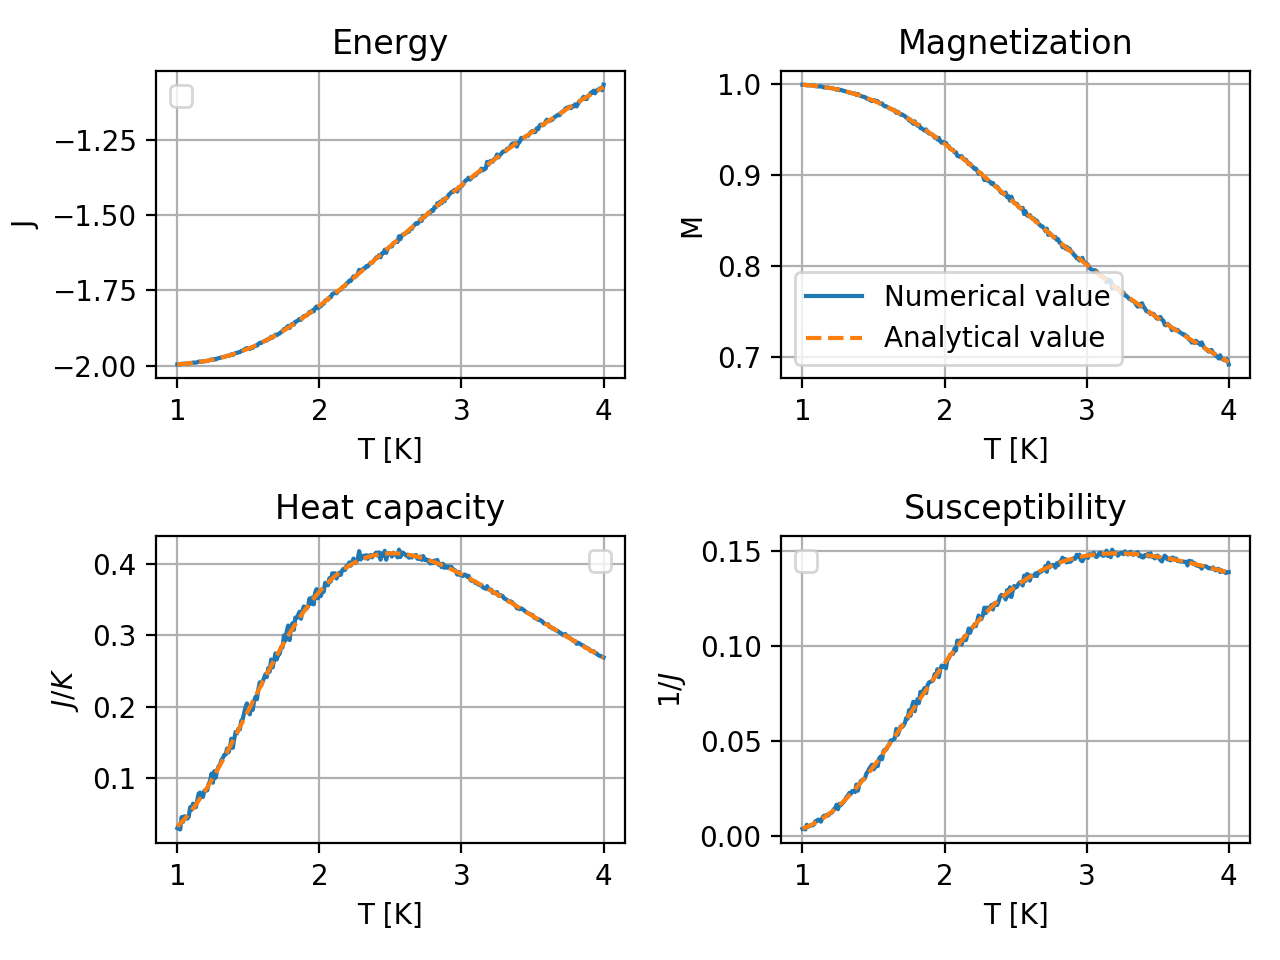
\includegraphics[width=\linewidth]{Exp_values_2x2_5e5.png}
	\caption{Analytical vs numerical for 2x2 lattice. }
	\label{fig:exp_val}
\end{figure}

\begin{figure}[H]
	\centering
	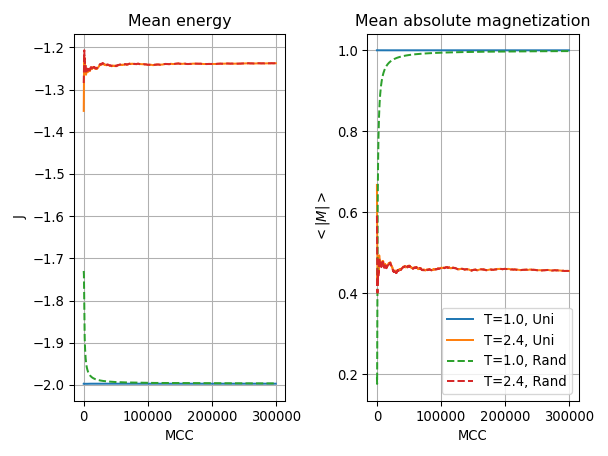
\includegraphics[width=\linewidth]{Uni_vs_rand.png}
	\caption{The mean energy and mean absolute magnetization.}
	\label{fig:mean_em}
\end{figure}

\begin{figure}[H]
	\centering
	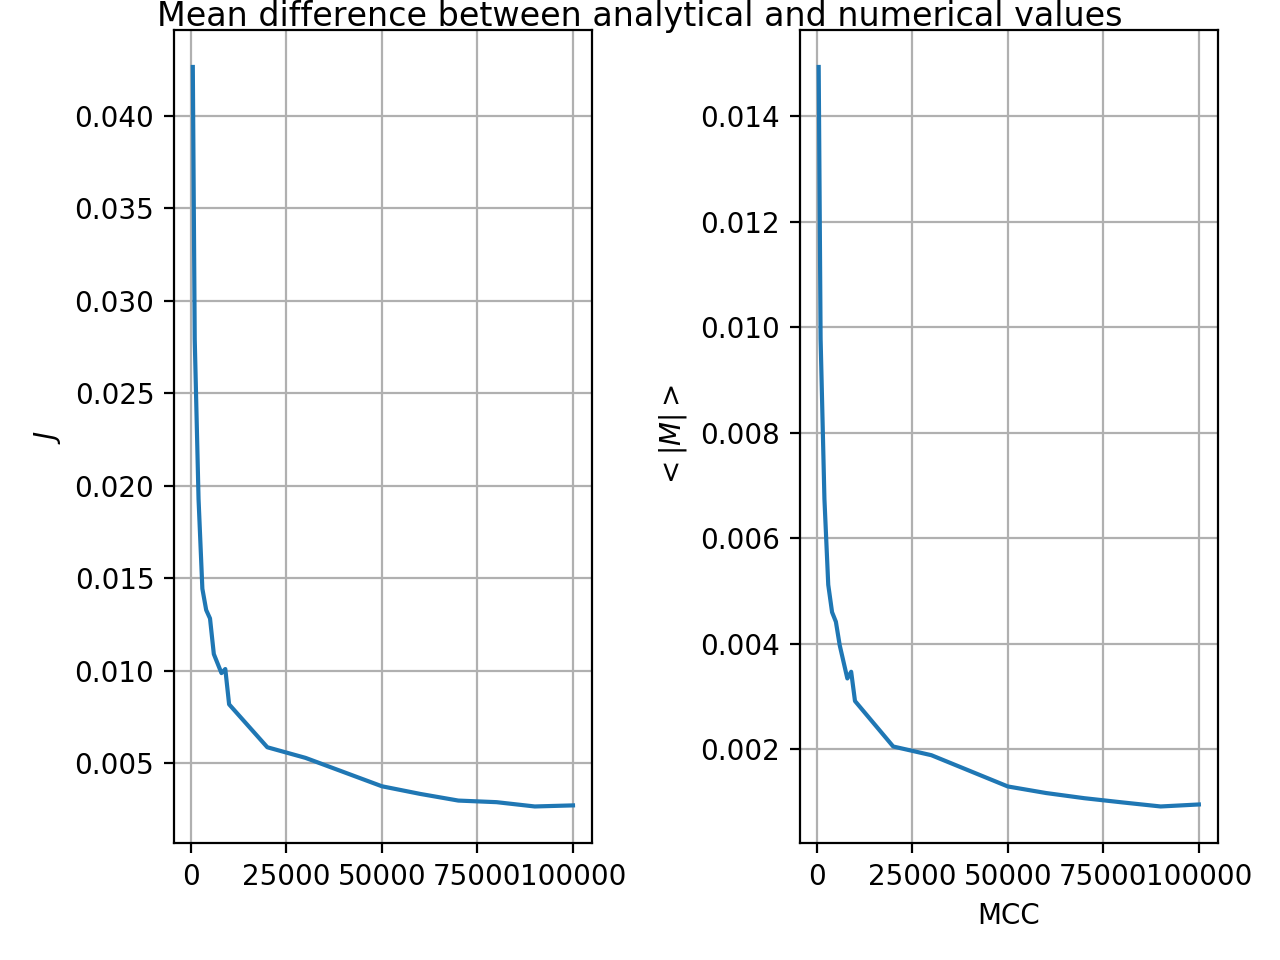
\includegraphics[width=\linewidth]{Diff_vs_mcs.png}
	\caption{Difference as a function of Monte Carlo cycles for $2\times2$ lattice.}
	\label{fig:diff_mc}
\end{figure}

\begin{figure}[H]
	\centering
	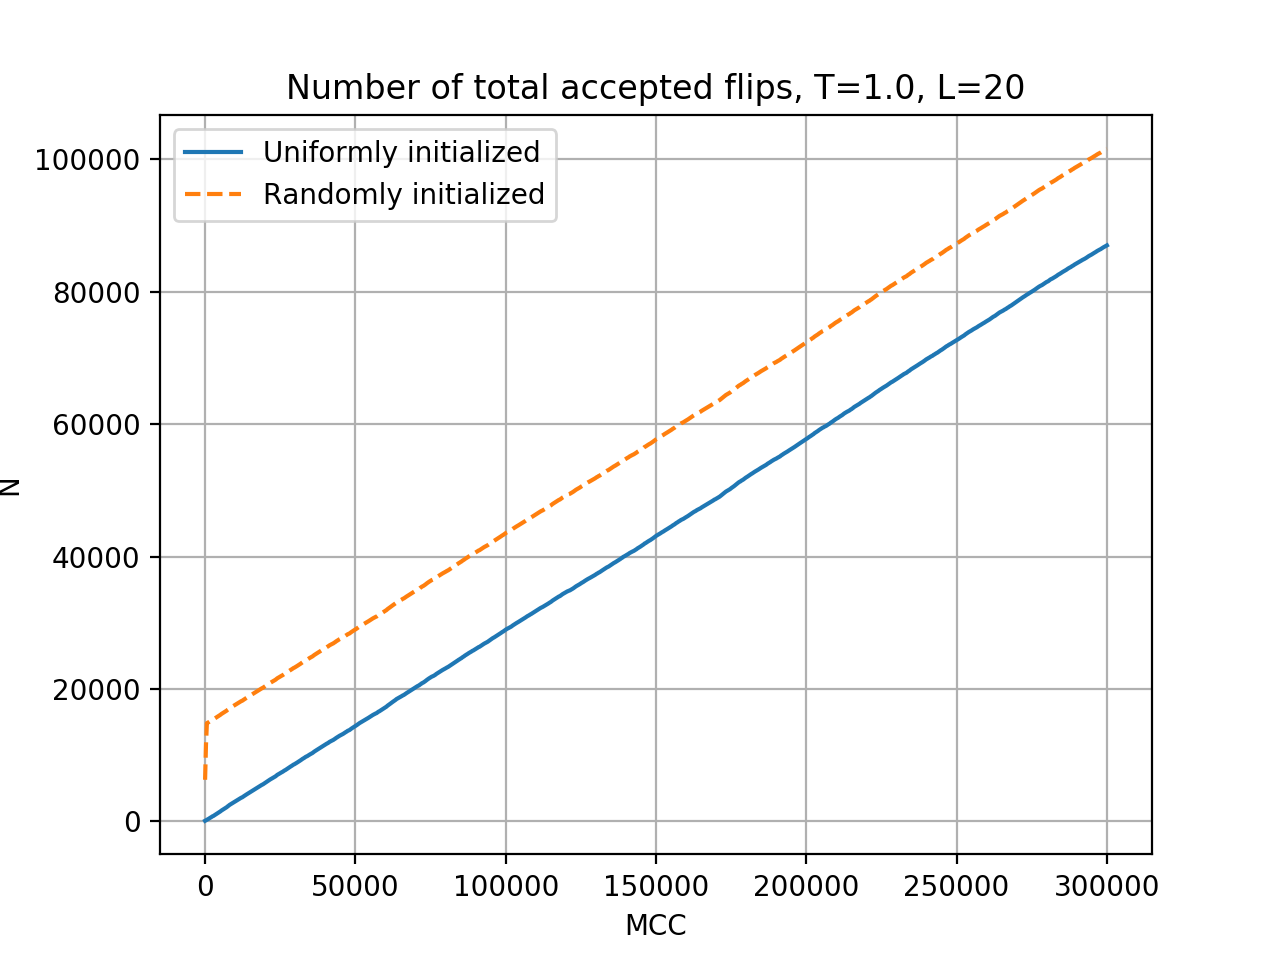
\includegraphics[width=100mm]{n_flips_1.png}
	\caption{Number of total accepted flips as a function of MCS for the temperature T=1.0.}
	\label{fig:n1}
\end{figure}

\begin{figure}[H]
	\centering
	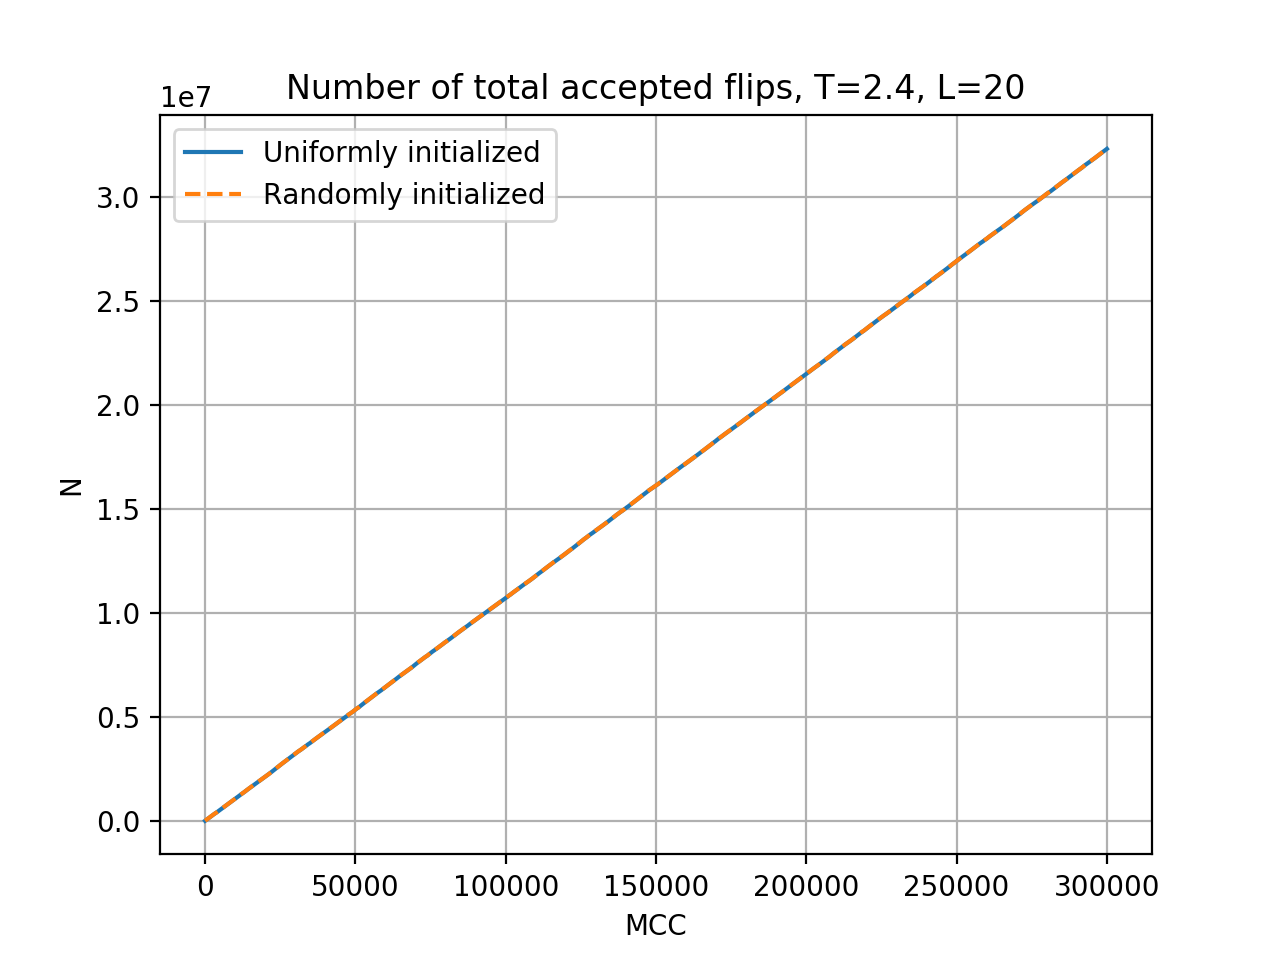
\includegraphics[width=100mm]{n_flips_24.png}
	\caption{Number of total accepted flips as a function of MCS for the temperature T=2.4.}
	\label{fig:n24}
\end{figure}

\begin{figure}[H]
	\centering
	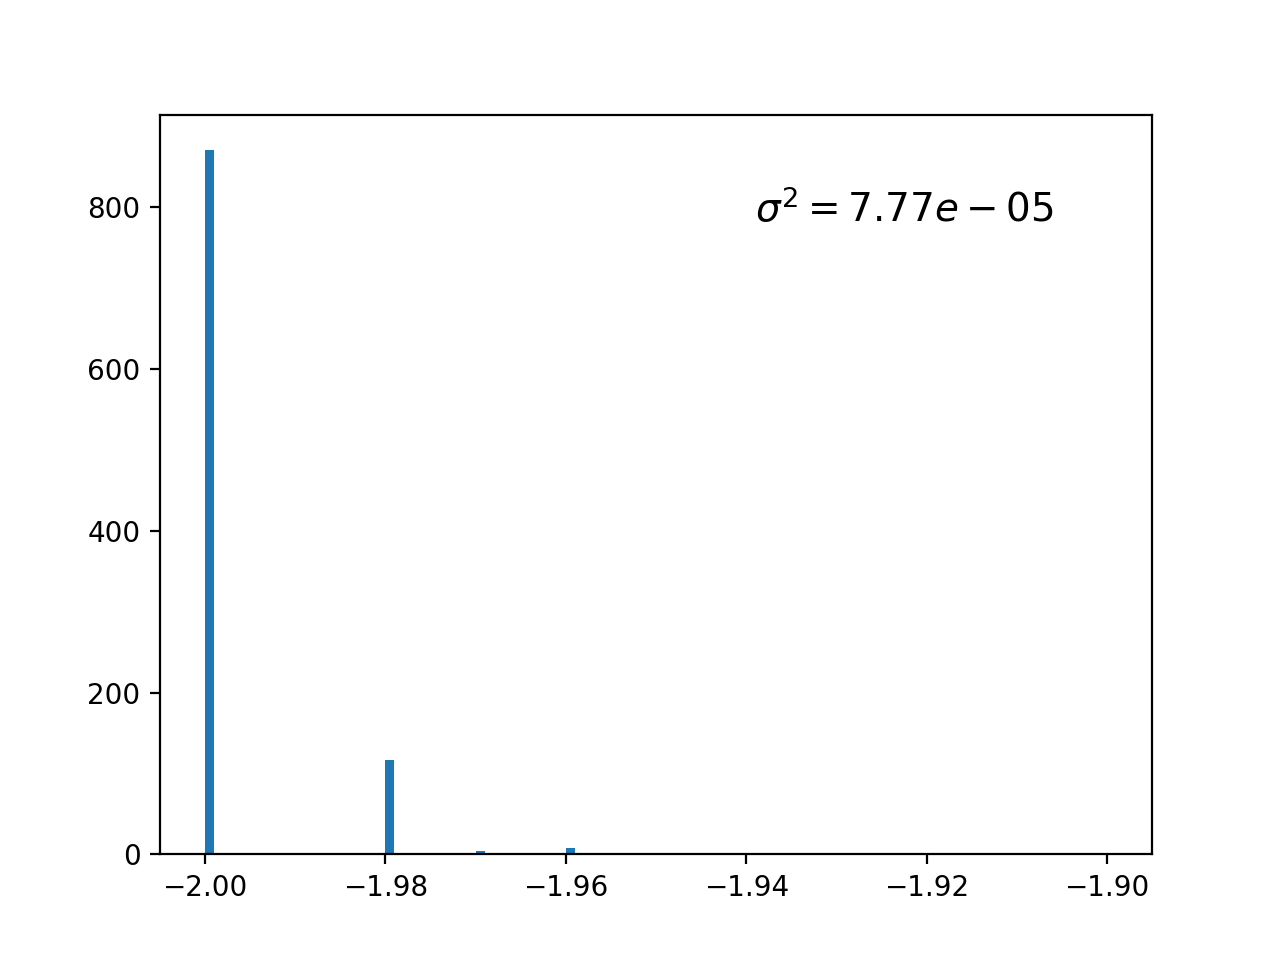
\includegraphics[width=100mm]{Hist_1.png}
	\caption{The probability distribution for the temperature T=1.0.}
	\label{fig:pd1}
\end{figure}

\begin{figure}[H]
	\centering
	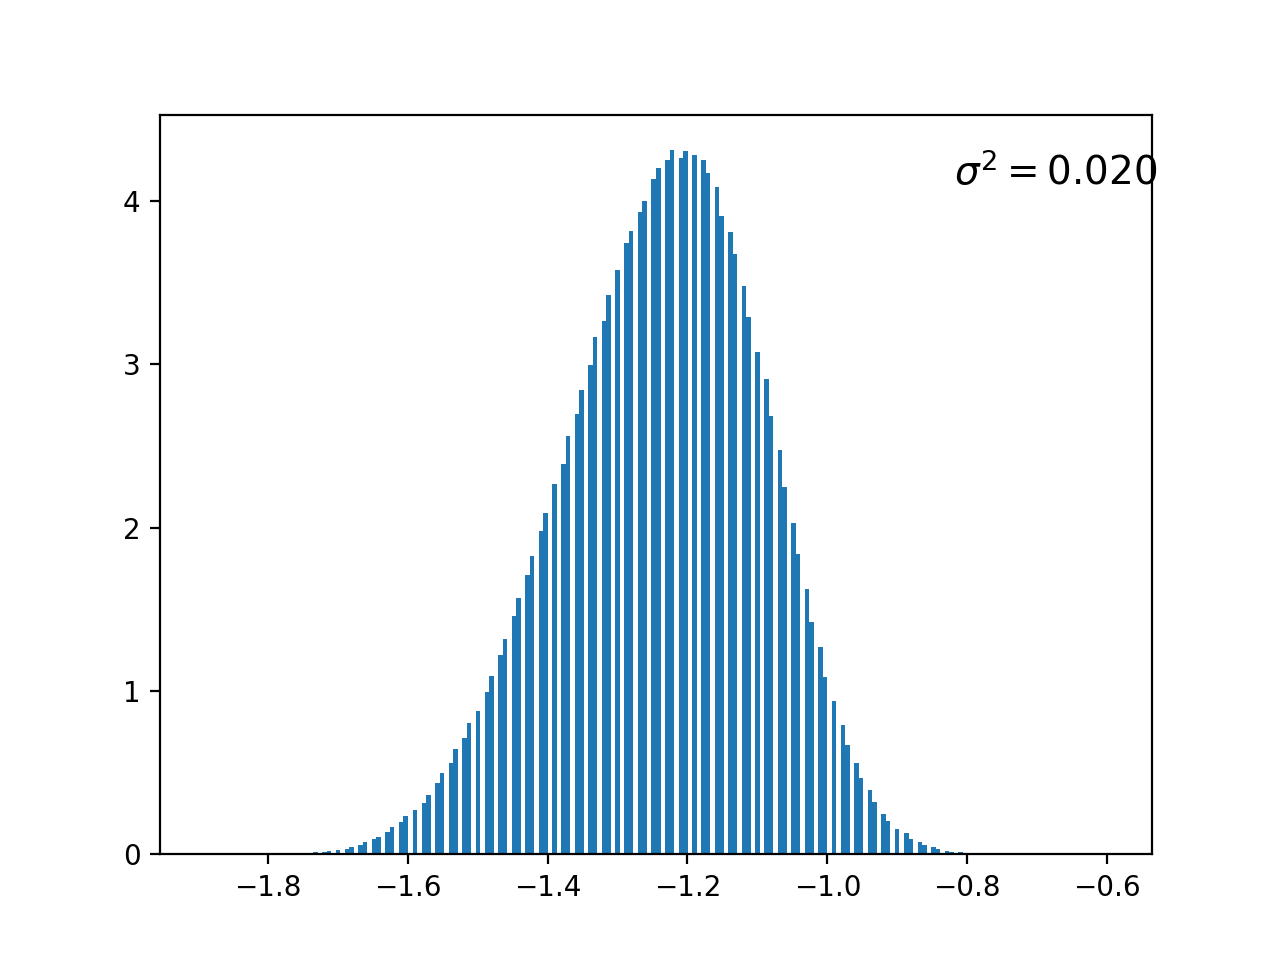
\includegraphics[width=100mm]{Hist_24.png}
	\caption{The probability distribution for the temperature T=2.4 J/k.}
	\label{fig:pd24}
\end{figure}

\begin{figure}[H]
	\centering
	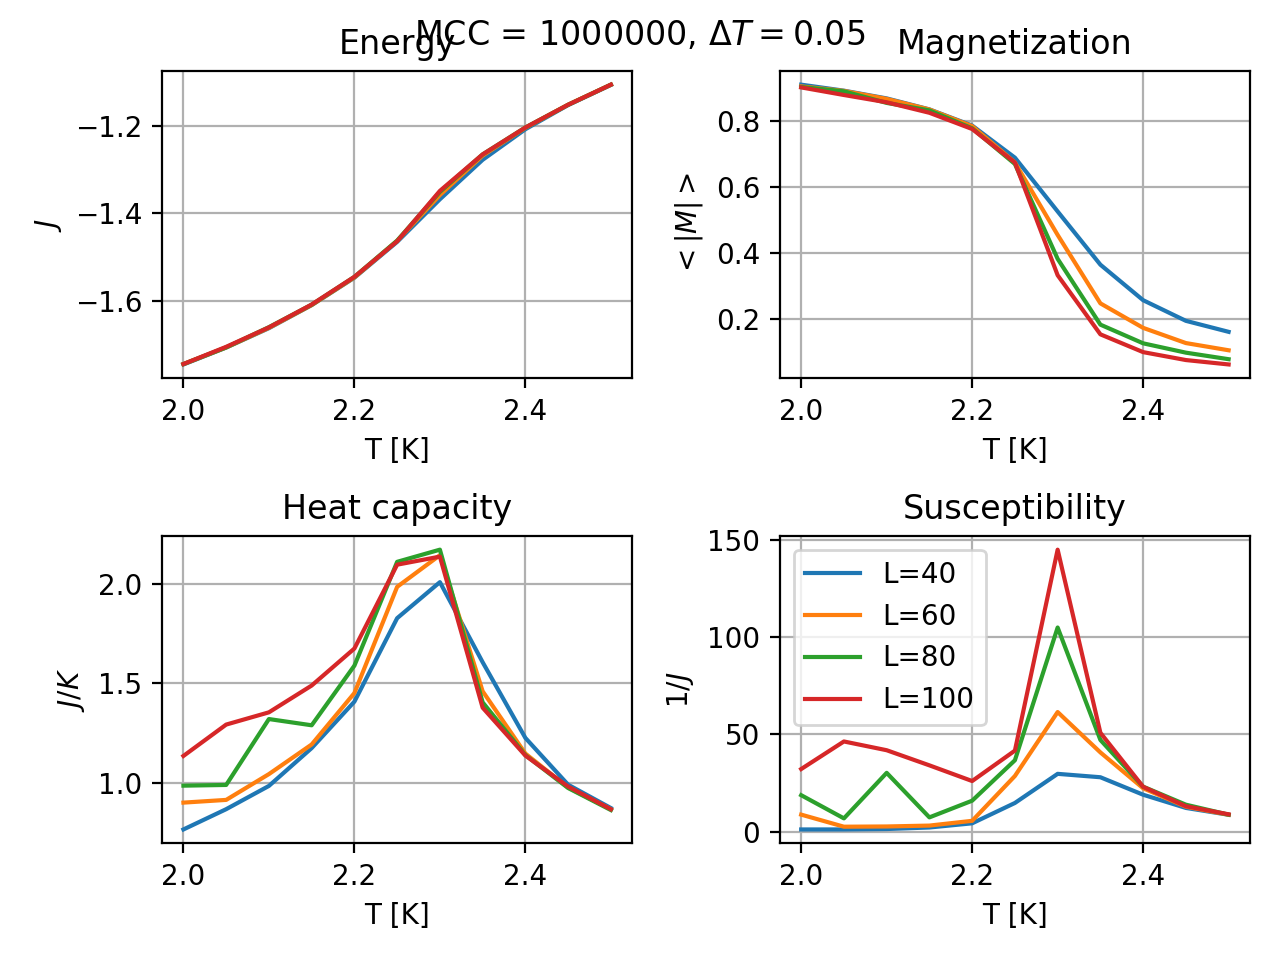
\includegraphics[width=\linewidth]{Exp_values.png}
	\caption{Expectation values for E, $|M|$, $C_V$ and $\chi$ as functions of T for L=40, L=60, L=80 and L=10.}
	\label{fig:exp}
\end{figure}

\begin{figure}[H]
	\centering
	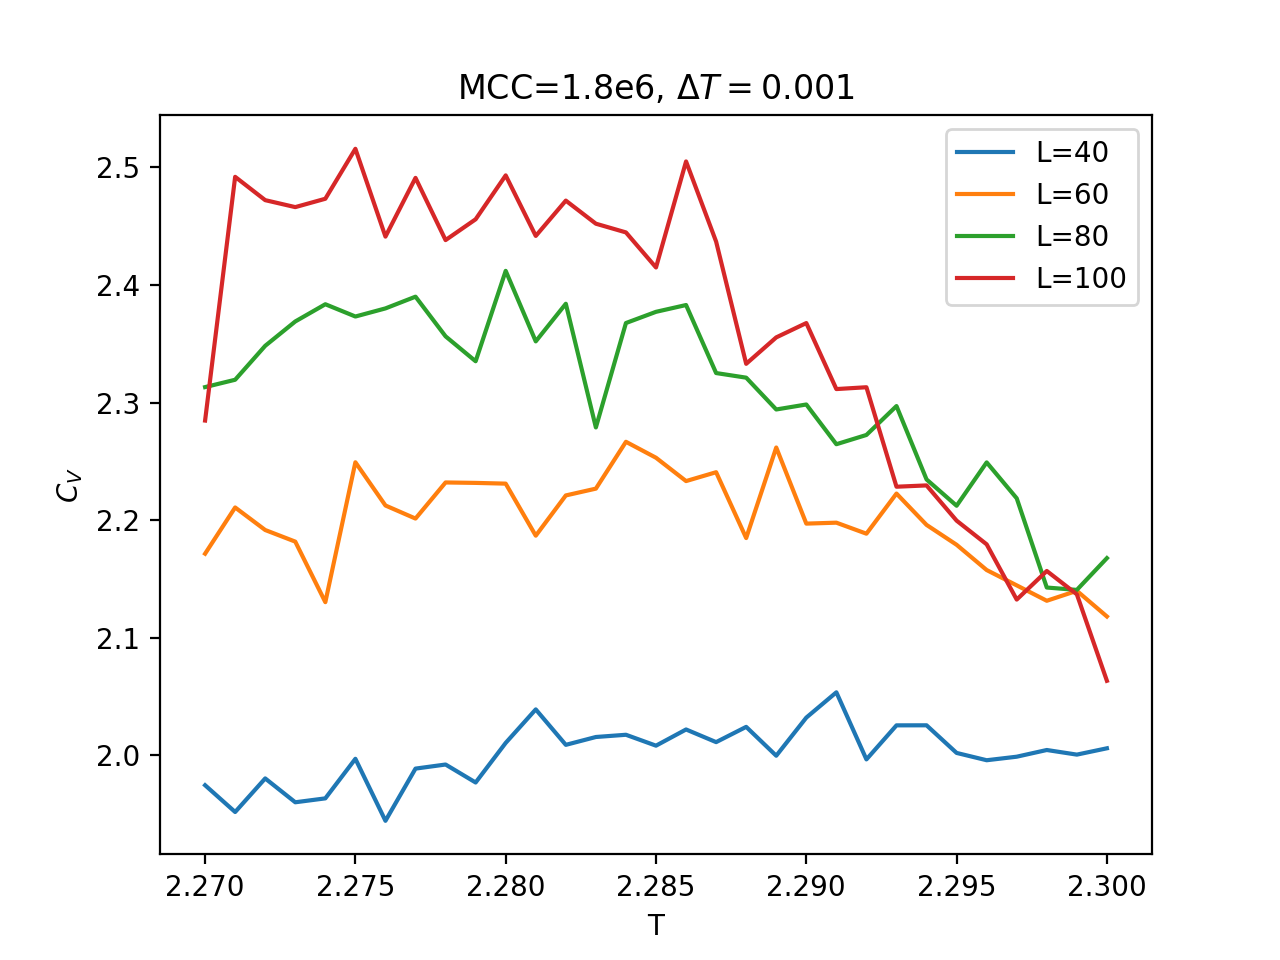
\includegraphics[width=100mm]{Exp_values_zoom.png}
	\caption{Heat capacity as a function of temperature over the critical temperature interval.}
	\label{fig:C_T}
\end{figure}

\subsection*{Illustrations}

\begin{figure}[H]
	\centering
	\includegraphics[width=100mm]{Spin}
	\caption{The different spin orientations.}
	\label{fig:spinn}
\end{figure}

\clearpage
\section{Appendix}
\subsection*{Analytical expressions}

We can use our analytical expressions in conjunction with periodic boundary conditions. We assume two spins in each dimension L=2. If we draw up each lattice with the different spin orientations we can find the degeneracy, energy and magnetization for each state. These values can be used to find the analytical expressions with periodic boundary conditions. We have five different spin orientations if we are studying the spin structures in Figure \ref{fig:spinn}. The energy differences $\Delta E$ in such a structure is given by equation \ref{eq:dM}. We can also find the difference in magnetization $\Delta M$ by using equation \ref{eq:dE}.

\begin{table}[H]
\begin{center}
\caption{Energy and magnetization given number of up spins.}
\begin{tabular}{  |c|c|c|c|c|c| } \hline
$N_{\text{spins up}}$&Degeneracy&E&M \\ \hline
4&1&-8 J&4\\ \hline
3&4&0 &2 \\ \hline
2&4&0&0\\ \hline
2&2&8 J&0\\ \hline
1&4&0&-2\\ \hline
0&1&-8 J&-4\\ \hline
\end{tabular}
\label{tab:up_spins}
\end{center}
\end{table}

In Table \ref{tab:up_spins} we have the energy and magnetization given the number of up spins. 

The partition function for the $2\times2$ lattice is given by equation \ref{eq:Z}:

\begin{equation}
\begin{split}
Z&=2e^{8J\beta}+2e^{-8J\beta}+12e^0\\
&=4\cosh{(8J\beta)}+12
\end{split}
\label{eq:calc_Z}
\end{equation}

This expression combined with equation \ref{eq:E_m} gives the energy:

\begin{equation}
\begin{split}
E_m &= \frac{2\times8Je^{-8J\beta}-2\times8Je^{8J\beta}}{Z}\\
&=\frac{-16J(e^{8J\beta}-e^{-8J\beta})}{Z}\\
&=\frac{-32J\sinh{(8J\beta)}}{Z}
\label{eq:calc_E}
\end{split}
\end{equation}

We also have a variance $<\sigma_E^2>$ which we find by using equation \ref{eq:E_v}:

\begin{equation}
\begin{split}
<\sigma_E^2>&=\bigg(\frac{(-8J)^2e^{-(-8\beta J)} + 2 \times (8J)^2e^{-(8\beta)}+(-8J)^2e^{-(-8\beta J)}}{Z}\bigg)-E_m^2\\
&=\frac{128J^2(e^{8J\beta}+e^{-8J\beta})}{Z}-E_m^2=\frac{256J^2\cosh{(8J\beta)}}{Z}-\bigg(\frac{-32J\sinh{(8J\beta)}}{Z}\bigg)^2
\label{eq:calc_Ev}
\end{split}
\end{equation}

Which gives us the heat capacity $C_v$ by using equation \ref{eq:C_v}:

\begin{equation}
C_v = \frac{1}{kTZ^2} \bigg(1024\beta J^2(3\cosh(8J\beta) + 1\bigg)
\label{eq:calc_Cv}
\end{equation}

We find the mean magnetization by using equation \ref{eq:mM}:

\begin{equation} \label{eq:calc_M}
\begin{split}
\langle M \rangle& = 1\times 4 \times P(-8) + 4 \times 2 \times P(0) + 4 \times 0 \\
& + 2\times0+4 \times (-2) \times P(0) +  1\times(-4) \times P(-8)\\
&=4\bigg(\frac{e^{-8J\beta }}{4\cosh{(8J\beta)}+12}\bigg)-4\bigg(\frac{e^{-8J\beta }}{4\cosh{(8J\beta)}+12}\bigg) \\
&=0
\end{split}
\end{equation}

We can also find the absolute value:

\begin{equation}
\begin{split}
\langle |M| \rangle &= \frac{1}{Z}\bigg(4e^{8J\beta}+4\times2e^0+4\times|-2|e^0+|-4|e^{8J\beta}\\
&=\frac{8}{Z}(e^{8J\beta}+2)
\label{eq:mean_calc_M}
\end{split}
\end{equation}


We also have a variance $<\sigma_M^2>$ which we find by using equation \ref{eq:M_v}:

\begin{equation}
\begin{split}
<\sigma_M^2>&=\frac{1}{Z}\bigg(4^2e^{-(-8J\beta)}+4\times 2^2e^0+4\times(-2)^2e^0+(-4)^2e^{-(-8\beta)}\bigg)\\
&=\frac{32}{Z}(1+e^{8J\beta})
\end{split}
\label{eq:calc_Mv}
\end{equation}

Which gives us the susceptibility $\chi$ by using equation \ref{eq:chi}:

\begin{equation}
\chi = \frac{1}{kT} \bigg(\frac{32}{Z}(1+e^{8J\beta})-\frac{64}{Z^2}(e^{8J\beta}+2)^2\bigg)
\label{eq:calc_chi}
\end{equation}

We assume that the original position of the middle spin in Figure \ref{fig:spinn} is up (the middle spin is the dot). We find the energy differences by using equation \ref{eq:dM}:

\begin{equation}\label{eq:calc_dE}
\begin{split}
&\Delta E_1 = 4-(-4)=8\\
&\Delta E_2 = 2-(-2)=4\\
&\Delta E_3 = -2-(2)=-4\\
&\Delta E_4 = 0-0=0\\
&\Delta E_5 = -4-(4)=-8\\
\end{split}
\end{equation}

We can see that we obtain five different energy differences as we flip the spin from up to down in the middle of the structures in Figure \ref{fig:spinn}.

\bibliography{References} % Kilder.
\begin{thebibliography}{9}
\bibitem{94}
	Jensen, M.H., 2015, Computational Physics Lecture Notes Fall 2015
\bibitem{95}
	Jensen, M.H., 2017, Computational Physics Lectures: Statistical physics and the Ising Model
\end{thebibliography}

\end{document}